\section{Illustrating the Transition Rules of the CRDT Semantics}

\begin{figure}[t]
  % \centering
  \begin{subfigure}[!ht]{.3\linewidth}
    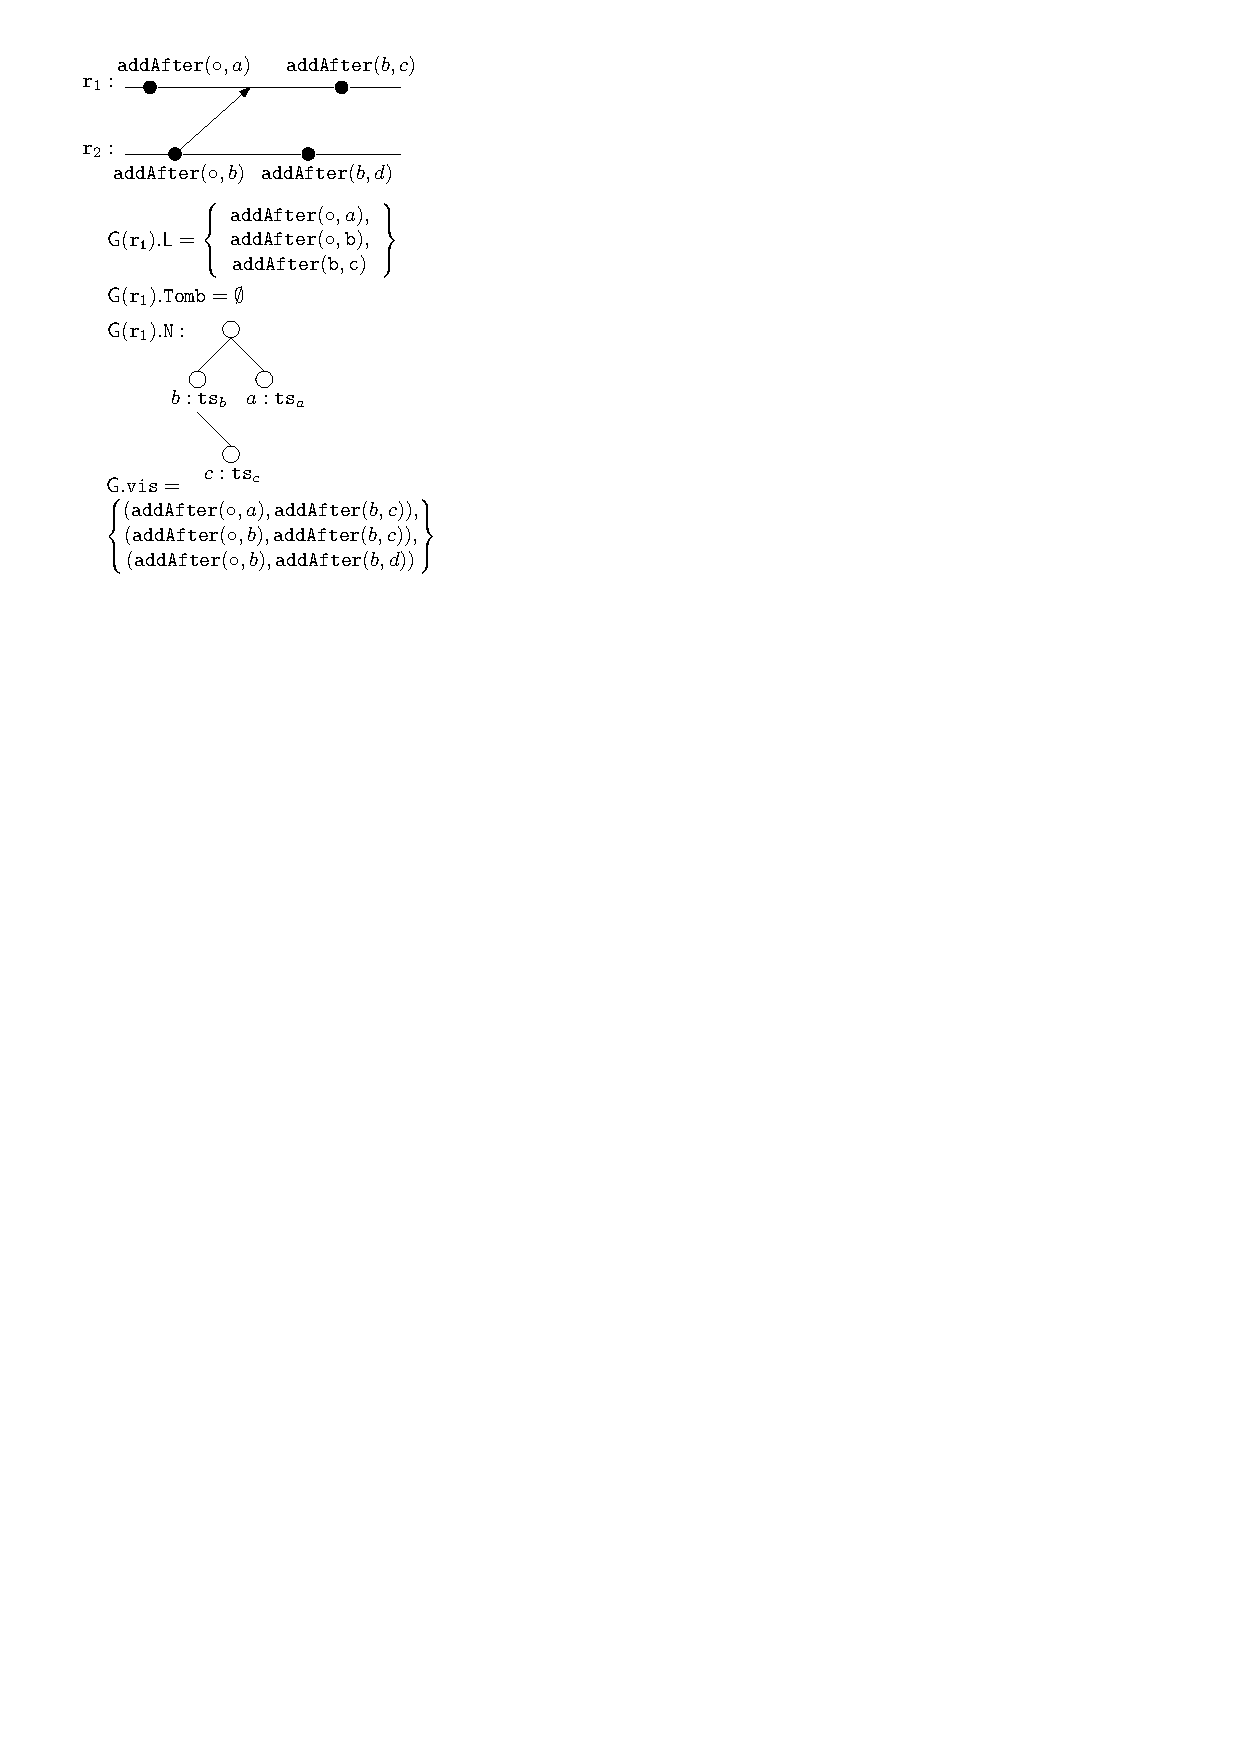
\includegraphics[scale=.7]{figures/LinRGA-1}
      \vspace{1.3cm}
    \caption{}
    \label{fig:rga-sem-1}
  \end{subfigure}
  \begin{subfigure}[!ht]{.3\linewidth}
      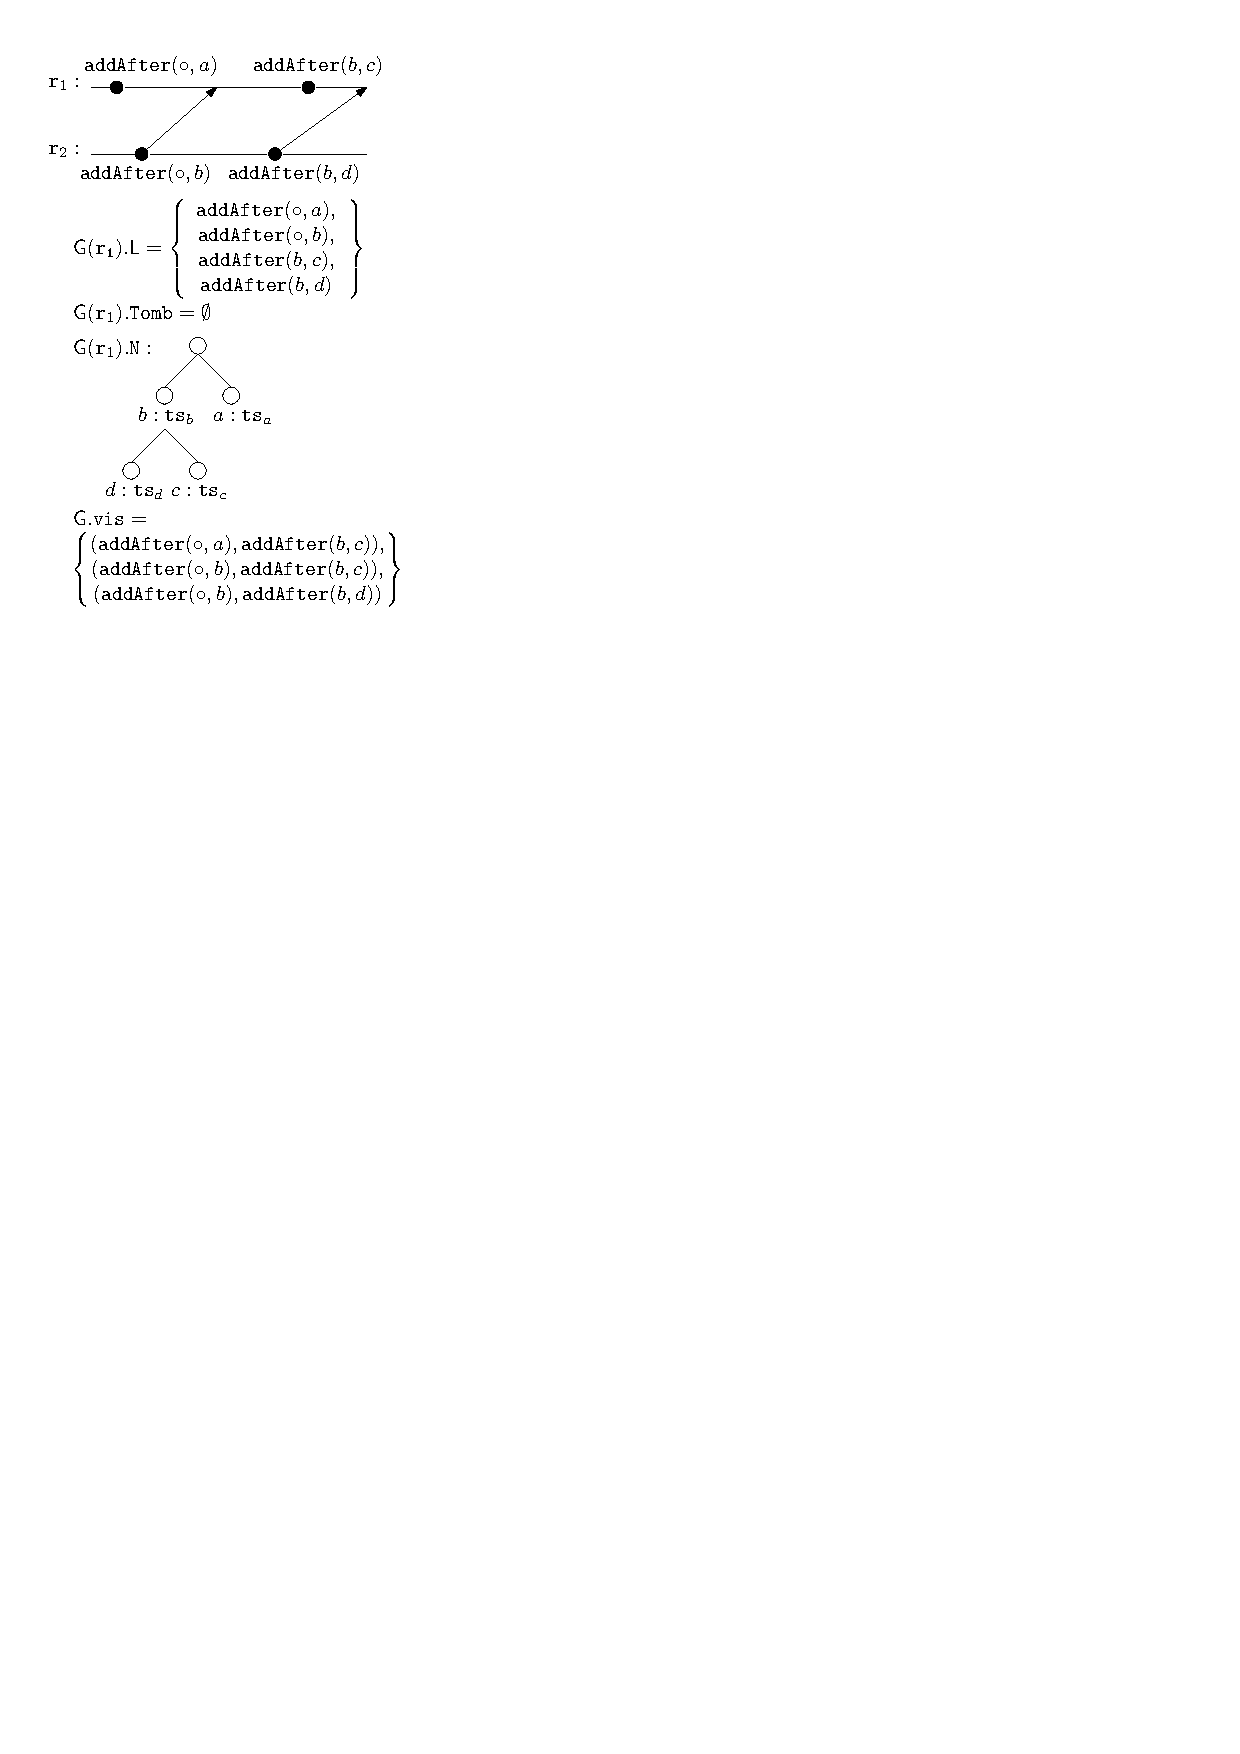
\includegraphics[scale=.7]{figures/LinRGA-2}
      \vspace{1cm}
    \caption{}
    \label{fig:rga-sem-2}
  \end{subfigure}
  \begin{subfigure}[!ht]{.3\linewidth}
    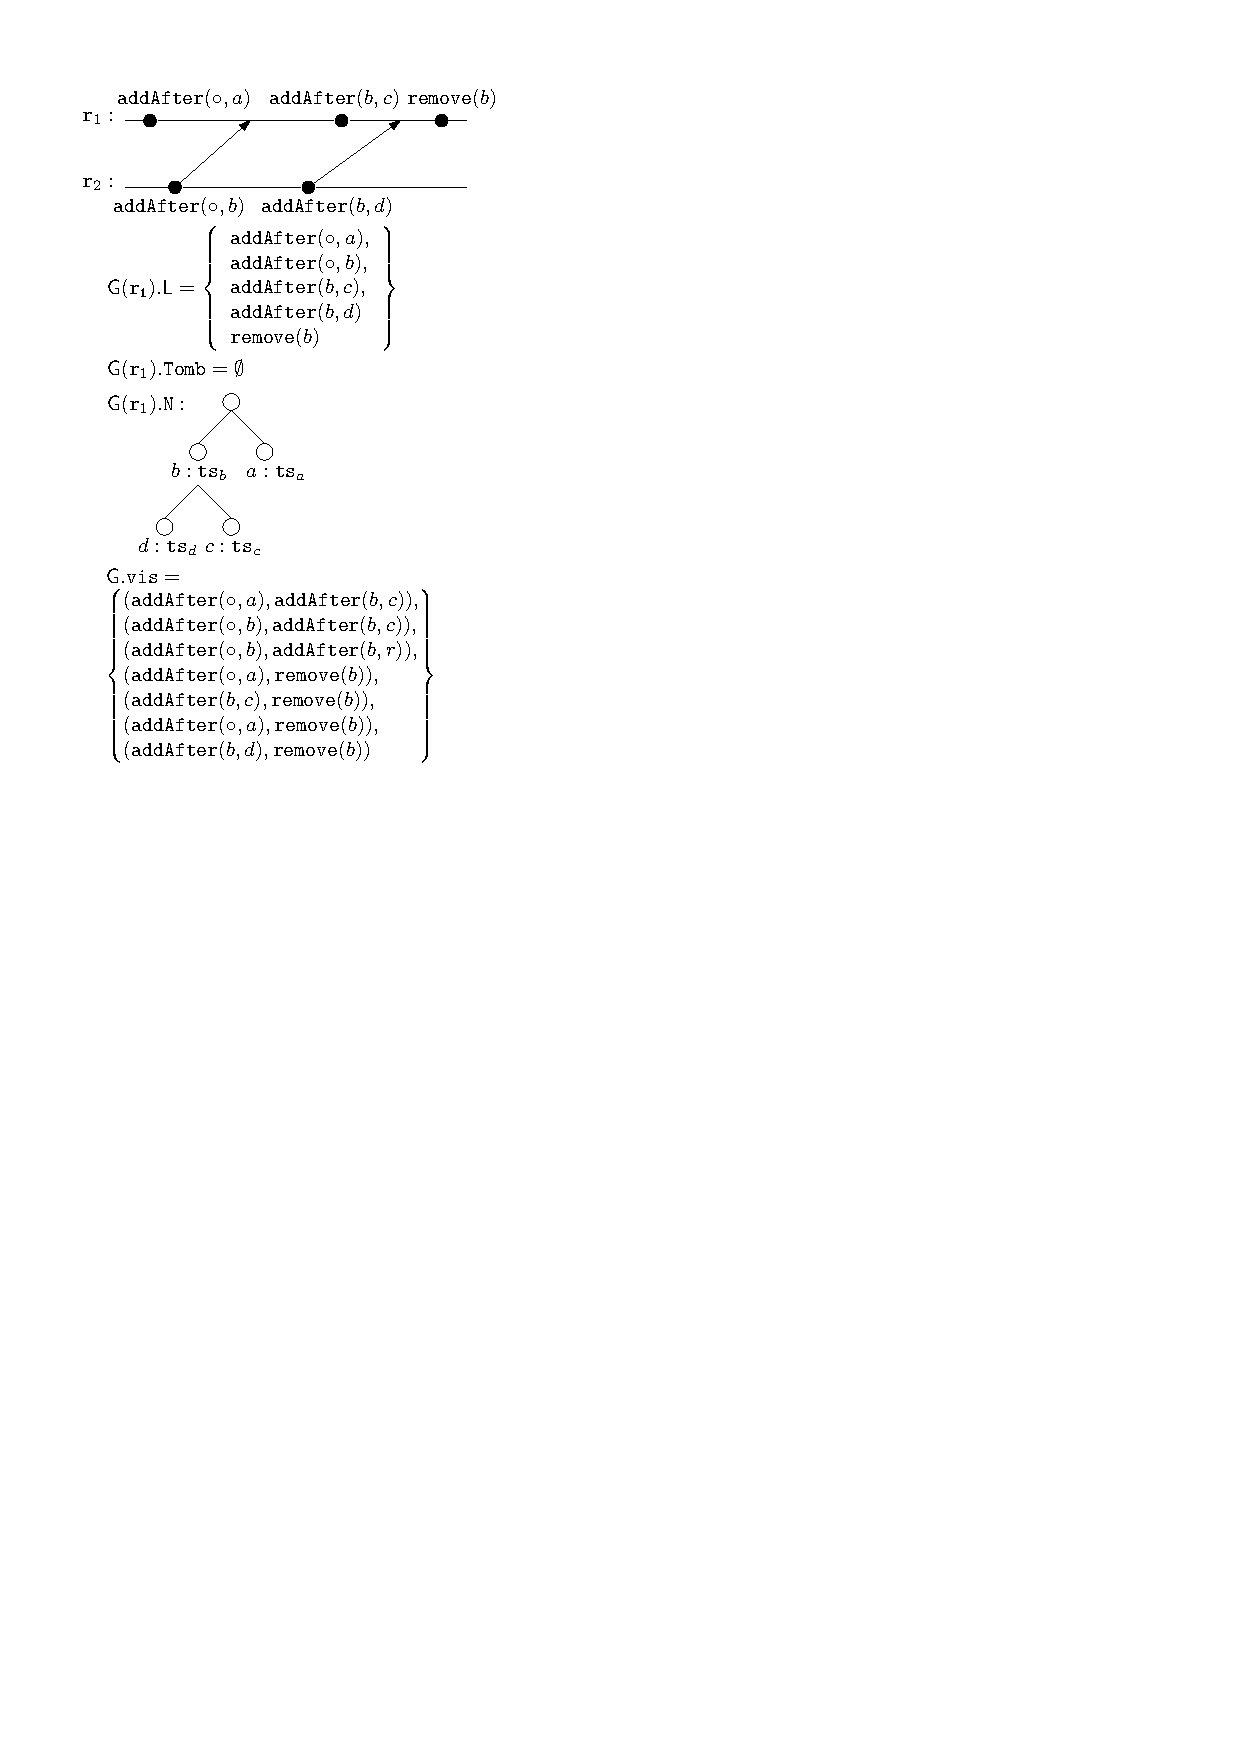
\includegraphics[scale=.7]{figures/LinRGA-3}
    \caption{}
    \label{fig:rga-sem-3}
  \end{subfigure}
  \caption{Example of the semantics of RGA.}
  \label{fig:rga-sem}
\end{figure}

\autoref{fig:rga-sem} shows how some components of the semantics
progress according to the rules of~\autoref{fig:crdt-opsem} for the
RGA data type.
%
In particular we shown: the local labels of replica $\arep_1$
($\gstates(\arep_1).\alabelset$); its state, where we remove the
$\astate$ for succinctness (then $\gstates(\arep_1).\astate.\mathsf{N}$
becomes $\gstates(\arep_1).\mathsf{N}$); and the global visibility
relation $\gstates.\mathtt{vis}$.
%
The transition from~\autoref{fig:rga-sem-2} to~\autoref{fig:rga-sem-3}
shows an {\sc Operation} transition where the operation
$\mathtt{remove}(b)$ is executed by replica $\arep_1$.
%
Notice in particular how the global visibility relation is extended.

In~\autoref{fig:rga-sem}, the transition from~\autoref{fig:rga-sem-1}
to~\autoref{fig:rga-sem-2} corresponds to a {\sc DownStream}
transition which extends the visibility of the operation
$\mathtt{addAfter}(b, d)$ to $\arep_1$.
%
Notice that this is reflected in the $\gstates(\arep_1).\alabelset$
component.
%
The relation $\gstates.\mathtt{vis}$ does not change since this
relation only changes when a new operation is executed at the source
replica.
